\documentclass[../report.tex]{subfiles}
\begin{document}	
	
\chapter{State of the art}
The most interesting aspect of fabricating optical waveguides from silicon is based on low primary cost of material, the mature and evolved manufacturing techniques owing to decades of research and the potential to develop monolithic \gls{ic} using the same substrate.

	\section{Theoretical background of SOI waveguide}
Although silicon is the optimal material for electronics, only recently silicon is being considered as a practical option for \gls{oeic} solutions. Silicon has many properties conducive to fiber optics. The band gap of silicon ($\sim$\SI{1.1}{\electronvolt}) is such that the material is transparent to wavelengths commonly used for optical transport ($\sim$\SI{1.3}{\micro\metre}-\SI{1.6}{\micro\metre}). One can use standard \gls{cmos} processing techniques to sculpt optical waveguides onto the silicon surface. Similar to an optical fiber, these optical waveguides can be used to confine and direct light as it passes through the silicon \cite{reed_silicon_2004}. Due to the wavelengths typically used for optical transport and silicon’s high index of refraction, the feature sizes needed for processing these silicon waveguides are on the order of \SI{0.5}{\micro\metre}-\SI{1}{\micro\metre}. The lithography requirements needed to process waveguides with these sizes exist today. If we push forward to leading-edge research currently under way in the area of \gls{pbg} devices, today’s state-of-the-art \SI{90}{\nano\metre} fabrication facilities should meet the technical requirements needed for processing \gls{pbg} devices. What this says is that we may already have all or most of the processing technologies needed to produce silicon-based photonic devices for the next decade. In addition, the same carriers used for the basic functionality of the transistor (i.e. electrons and holes) can be used to modulate the phase of light passing through silicon waveguides and thus produce ‘active’ rather than passive photonic devices. Finally, if all this remains \gls{cmos}-compatible, it could be possible to process transistors alongside photonic devices, the combination of which could bring new levels of performance, functionality, power and size reduction, all at a lower cost.
		
		\subsection{Maxwell's equations}
Light is high frequency \gls{em} phenomenon having wave-particle duality. Visible light, ultraviolet light, and infrared light are all electromagnetic waves of differing frequency. 
\begin{figure}[h]
	\centering
	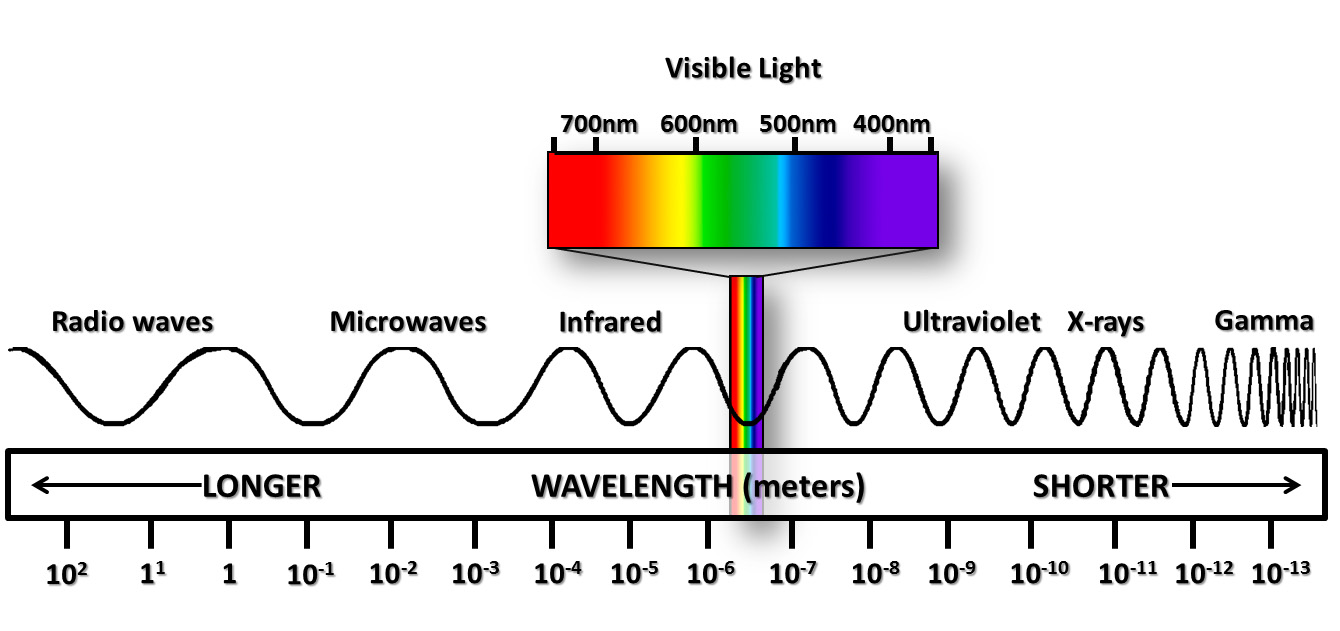
\includegraphics[width=0.75\textwidth]{2-light-spectrum}
	\caption{The \gls{em} wave spectrum}
	\label{fig:2_light_spectrum}
\end{figure}
James Clerk Maxwell discovered that he could combine four simple equations, which had been previously discovered, along with a slight modification to describe self-propagating waves of oscillating electric and magnetic fields \cite{waveparticle_2016}. The understanding of propagating of light waves using Maxwell's equations in a dielectric medium, is the key to the construction of silicon waveguides. Maxwell’s equations relate the electric field $E$ (V/m), magnetic field $H$ (A/m), charge density $\rho$ (C/m3), and current density $J$ (A/cm2).
\begin{itemize}	
	\item \textbf{Maxwell's first equation (Gauss' Law)}: The net electric flux through any closed surface is equal to $\frac{1}{\epsilon_m}$ times the charge density within that closed surface.
	\begin{equation}\label{eq:max1_1}
	\nabla.E = \frac{\rho}{\epsilon_m}	
	\end{equation}
	where $\epsilon_m$ the permittivity of the medium, and del operator, $\nabla$, is given by:
	\begin{equation}\label{eq:max1_2}
	\nabla = \left(\frac{\partial i}{\partial x},\frac{\partial j}{\partial y},\frac{\partial k}{\partial z}\right)
	\end{equation}
	where i, j and k are unit vectors in the x, y and z directions respectively.
	
	\item \textbf{Maxwell's second equation (Gauss' Law for magnetic field)}: The net magnetic flux through a closed surface is always zero since magnetic monopoles do not exist.
	\begin{equation}\label{eq:max1_3}
	\nabla.H = 0	
	\end{equation}
	
	\item \textbf{Maxwell's third equation (Faraday's law)}: Induced electric field around a closed path is equal to the negative of the time rate of change of magnetic flux enclosed by the path.
	\begin{equation}\label{eq:max1_4}
	\nabla\times E = -\mu_m\frac{\partial H}{\partial t}
	\end{equation}
	where $\mu_m$ is the permeability of the medium.
	
	\item \textbf{Maxwell's fourth equation (Modification of Ampere's law)}:  The fourth equation states that magnetic fields can be generated in two ways: by electric current (this was the original "Ampere's law") and by changing electric fields (this was "Maxwell's addition") \cite{wiki_maxwells_2016}.
	\begin{equation}\label{eq:max1_5}
	\nabla\times H =  J + \epsilon_m\frac{\partial E}{\partial t}	
	\end{equation}	
\end{itemize}

All these equations combine into a simple wave equation after some mathematical calculations.
\begin{equation}\label{eq:wave_eq}
\nabla^2 E -  \mu_m\epsilon_m\frac{\partial^2 E}{\partial t^2} = \mu_m\frac{\partial J}{\partial t} + \frac{\nabla\rho}{\epsilon_m}	
\end{equation}
using the curl of curl identity operation given by: 
\begin{equation}\label{eq:curl_of_curl}
\nabla^2 E = \nabla(\nabla.E) - \nabla\times(\nabla\times E)
\end{equation}
A general solution to the equation \ref{eq:wave_eq} in free space, in absence of charge gives the following solution:
\begin{equation}\label{eq:wave_sol_electric}
\overrightarrow{E}(z,t)=E_{0}(x,y)e^{i\left(k_{0}z\pm \omega t\right)}
\end{equation}
where $z$ is direction of propagation of wave in Cartesian coordinates , phase ($\phi$) = $\left(k_{0}z\pm \omega t\right)$ and wave vector propagation constant ($k_0$) = $\dfrac {\partial \phi } {\partial t}$ = $\dfrac {2\pi } {\lambda }$, in the direction of propagation of the wave. It is worth mentioning that propagation constant in medium varies according to $n$, the effective \gls{ri} of the medium and is given by: 
\begin{equation}\label{eq:ri_med_val}
k = nk_0
\end{equation}
Similar calculations for the magnetic field, $H$ in free space yields, 		
\begin{equation}\label{eq:wave_sol_magnetic}
\overrightarrow{H}(z,t)=H_{0}(x,y)e^{i\left(k_{0}z\pm \omega t\right)}
\end{equation}

		\subsection{Eigenvalue and wave modes}
In general, the electric field in the wave equation in \ref{eq:wave_sol_electric} can be written in its constituent parts in Cartesian coordinates as:
\begin{equation}\label{eq:e_field_cart_cord}
\overrightarrow{E}=E_{x}i+E_{y}j+E_{j}k
\end{equation}
If the wave propagates towards z-direction through any waveguide medium and is a \gls{tem} wave front then we will have a constant electric field vector in the z-direction. In this case there will be different solutions for the propagation constant, $k$ in x and y directions. Now for each solution we can also get certain discrete angles at which the electric field can travel through the medium, which infers that light can propagate only at certain discrete angles through any dielectric medium. Each allowed solution is referred to as the \textit{mode of propagation} and are basically the different eigenvalues of the propagation vector. In the Fig. \ref{fig:2_em_wave} the electric field and magnetic field propagate in directions perpendicular to each other. Moreover, the direction of propagation is also transverse to the \gls{em} field. Hence it is called \gls{tem} wave.
\begin{figure}[H]
	\centering
	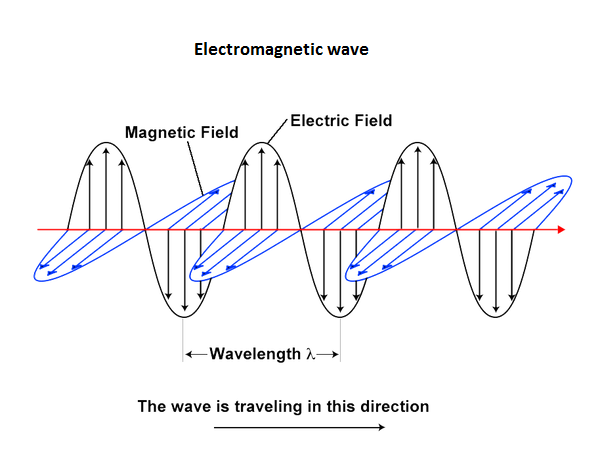
\includegraphics[width=0.75\textwidth]{2-em-wave}
	\caption{Propagation of \gls{em} wave}
	\label{fig:2_em_wave}
\end{figure}
\begin{figure}[H]
	\centering
	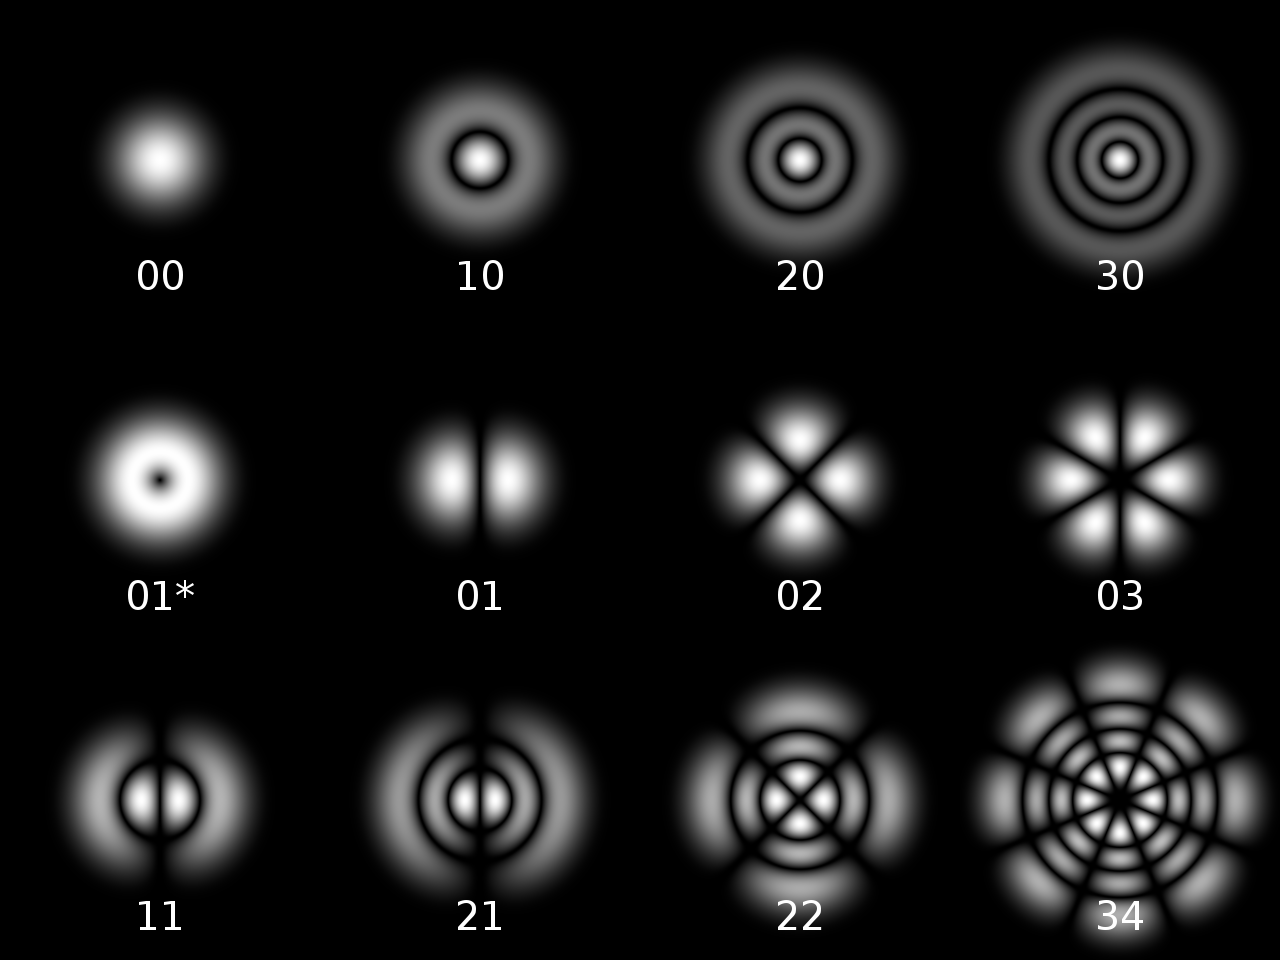
\includegraphics[width=0.75\textwidth]{2-modes}
	\caption{Propagation modes in optical fiber}
	\label{fig:2_modes}
\end{figure}
The eigenvalues provide the different acceptance angles at which light can be inserted into the waveguide resulting in different modes in the waveguide. Depending on various angles of incidence on the waveguide and the dimensions of the waveguide, various modes can be found which are basically the different eigenvalues of the wave solution \ref{eq:wave_sol_electric} and \ref{eq:wave_sol_magnetic}. For example, when light travels through optical fibers different modes can be visualized as follows in Fig. \ref{fig:2_modes}.
\todo{May be update the picture using CST}
		\subsection{Optical polarization and transverse modes}
Generally light in randomly polarized. Any kind of randomness is inefficient for data transmission. Optical fibers generally operate at \SI{1550}{\nano\metre} in fundamental \gls{te} or \gls{tm} mode. The ultimate goal of the on chip fabricated waveguide is to integrate with the currently deployed optical fiber network in a seamless manner. Hence, the waveguides must cater polarization into its design.  
\begin{figure}[h]
	\centering
	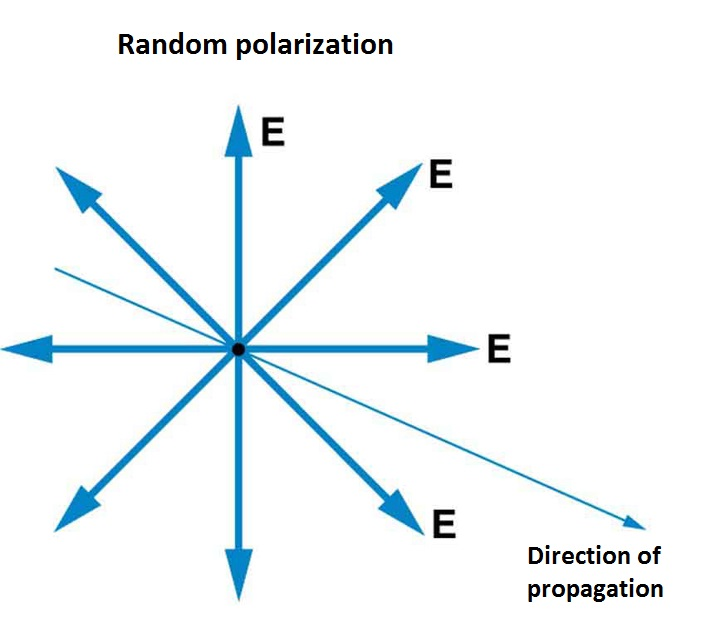
\includegraphics[width=0.75\textwidth]{2-random-pol}
	\caption{Random polarization of light}
	\label{fig:2_random_pol}
\end{figure}
\textit{Polarization} is the direction of the electric field associated with the propagating wave. However, the associated magnetic field is not always considered in the quantum domain for wave propagating at \SI{1550}{\nano\metre}. In the example in Fig. \ref{fig:2_em_wave} the wave is polarized since the electric field and magnetic field exist in one direction only. In a semiconductor optical waveguide light propagates in plane polarized modes and the plane in which light is polarized is either vertical or horizontal to the waveguide surface as shown in Fig. \ref{fig:2_te_tm_mode}. 
\begin{figure}[H]
	\centering
	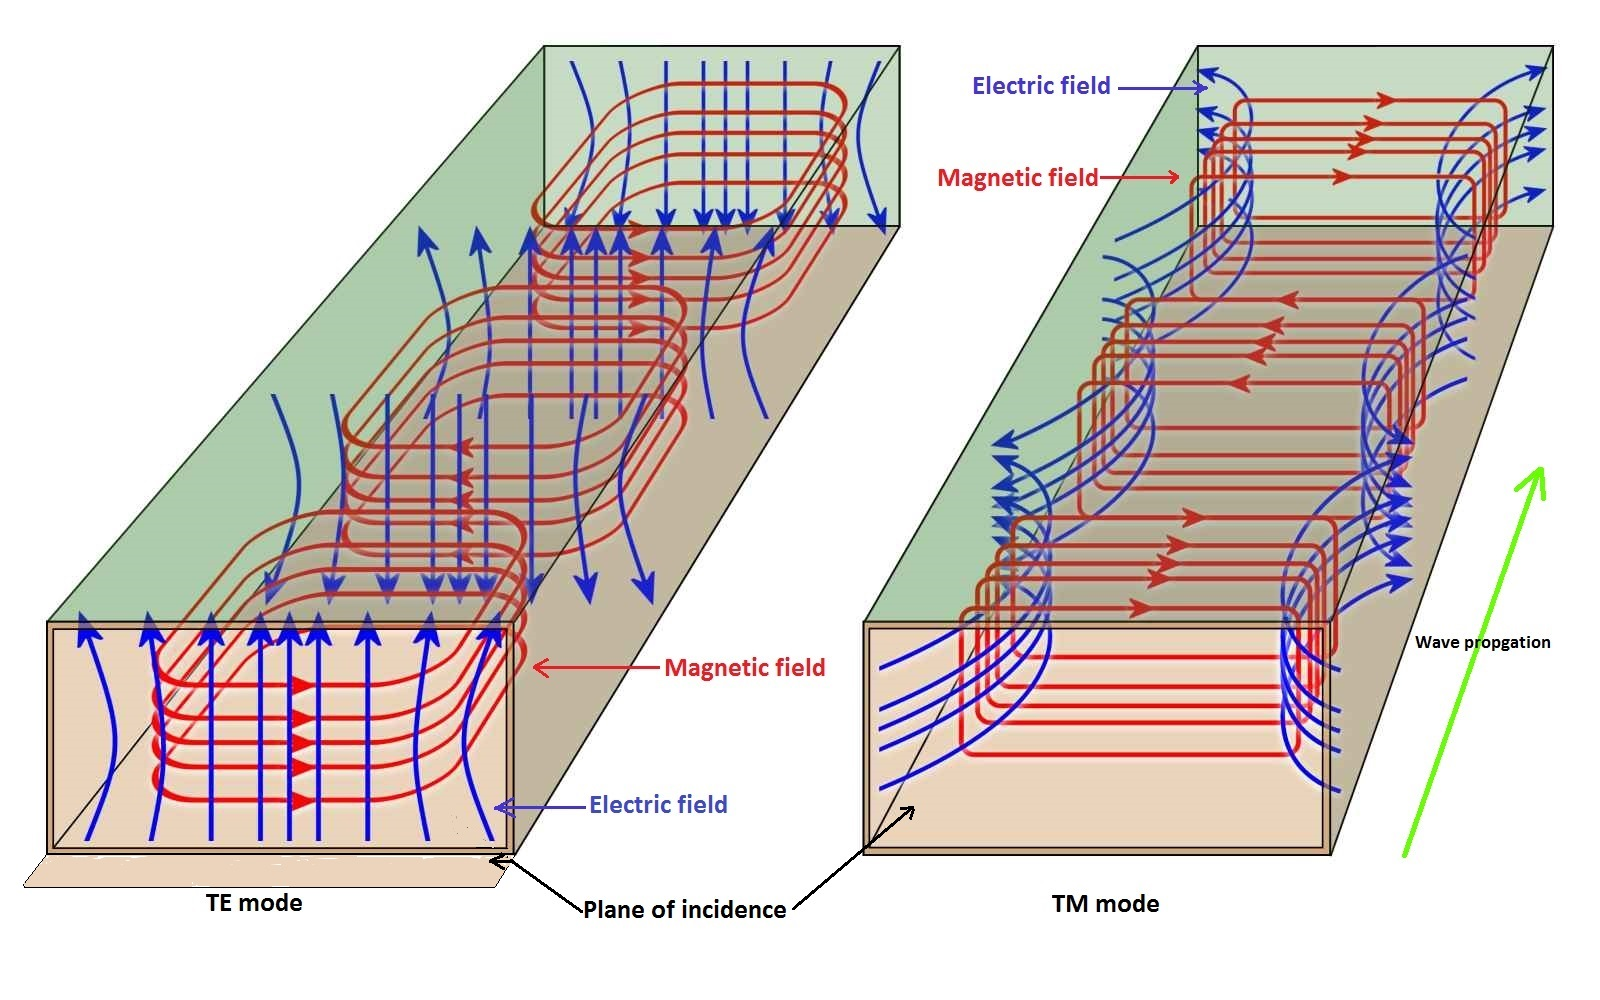
\includegraphics[width=0.75\textwidth]{2-te-tm-mode}
	\caption{\gls{te} and \gls{tm} modes in a waveguide}
	\label{fig:2_te_tm_mode}
\end{figure}			
			\subsubsection{TE mode}
\gls{te} mode is the fundamental mode in which electric field is perpendicular to the plane of incidence of light. As depicted in Fig. \ref{fig:2_te_tm_mode} it can be visualized that electric field lines shown by the blue lines are perpendicular to the plane of incidence in \gls{te} mode. The plane of incidence is the plane in which optical waves strike the surface of the waveguide.						
			\subsubsection{TM mode}
\gls{tm} mode is the fundamental mode in which magnetic field is perpendicular to the plane of incidence of light. As shown in Fig. \ref{fig:2_te_tm_mode} it can be visualized that magnetic field shown by the red lines are perpendicular to the plane of incidence in \gls{tm} mode.			
		
		\subsection{Optical waveguides}
Waveguide is the essential element of every photonic circuit which can be characterized by the number of dimensions in which light is confined inside it \cite{reed_silicon_2008}. A planar waveguide confines light in 1-D which is simple for understanding of the wave propagation using Maxwell's equations. However, for practical applications 2-D confinement is necessary and that is why channel waveguides are used. Structures like photonic crystals even have 3-D confinement properties.   			
			\subsubsection{Planar waveguides}
A simple planar waveguide consists of a high-indexed medium with height $h$	surrounded by lower indexed materials on the top and bottom sides. The \gls{ri} of the film, $n_f$ (generally made from Si) is greater than the \gls{ri} of the materials on the other sides. The \gls{ri} of the substrate in lower cladding is $n_s$, (generally made from SiO$_{2}$) whereas, \gls{ri} of the substrate in upper cladding is $n_c$ (generally which is air).
\begin{figure}[H]
	\centering
	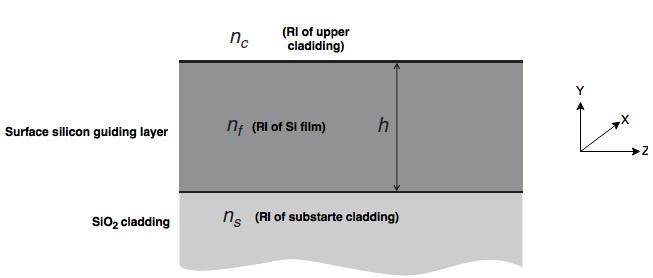
\includegraphics[width=0.75\textwidth]{2-palne-wg}
	\caption{A typical planar waveguide where the film is infinite in XZ-plane}
	\label{fig:2_palne_wg}
\end{figure}
For planar waveguides the wave equation for electric field \ref{eq:wave_sol_electric} and magnetic field can be rewritten as \ref{eq:wave_sol_magnetic} follows:
\begin{equation}\label{eq:wave_sol_planar_wg}
	\begin{aligned}
	\overrightarrow{E}(z,t)=E_{x}(y)e^{i\left(k_{0}z\pm \omega t\right)}\\
	\overrightarrow{H}(z,t)=H_{x}(y)e^{i\left(k_{0}z\pm \omega t\right)}
	\end{aligned}
\end{equation}	
since in X-direction the film is infinite. After using the homogeneous wave equations for a planar waveguide the following \gls{te} and \gls{tm} mode equations can be deduced:
\begin{equation}\label{eq:homogeneous_wave_sol_planar_wg}
	\begin{aligned}
	\nabla^{2}E_x(y) + (k_{0}^{2}n(y)^{2}-k^{2}){E_{x}(y)} = 0\\
	\nabla^{2}H_x(y) + (k_{0}^{2}n(y)^{2}-k^{2}){H_{x}(y)} = 0	
	\end{aligned}
\end{equation}
where \gls{ri} depends only on a single Cartesian coordinate $n = n(y)$. These equations can be solved using the various boundary conditions of the waveguides which help in deducing the nature of propagation of the wave in \gls{te} and \gls{tm} mode. Different kinds of numerical methods like \gls{fem}, \gls{fdtd}, \gls{bpm} have been developed to decipher the nature of light propagation in waveguides.
			\subsubsection{Channel waveguides}			
As mentioned earlier channel waveguides provide confinement in 2-D which helps in depicting more practical waveguides. The three main types of channel waveguides are rib, strip and buried waveguides. As depicted in \ref{fig:2_rib_wg}, \ref{fig:2_strip_wg}, \ref{fig:2_buried_wg} the different conceptual structures of the waveguides can be envisaged. While the rib and strip waveguides are designed using etching technique, the buried waveguide mostly relies on diffusion and epitaxial growth technique for its fabrication.
\begin{figure}[H] %h
	\begin{subfigure}[t]{0.3\textwidth}
		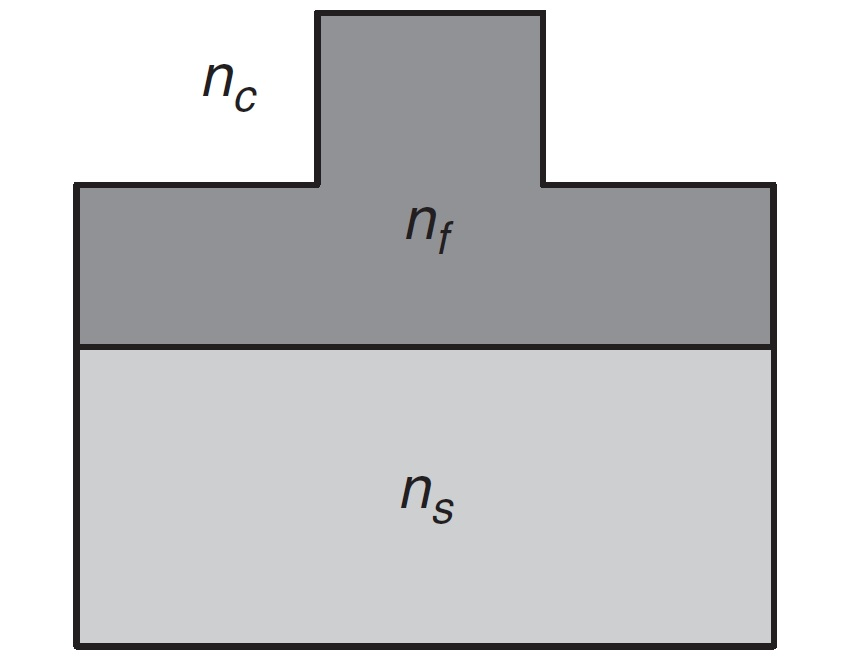
\includegraphics[width=\textwidth]{2-rib-wg}
		\caption{Rib waveguide}
		\label{fig:2_rib_wg}
	\end{subfigure}
	\hfill
	\begin{subfigure}[t]{0.3\textwidth}
		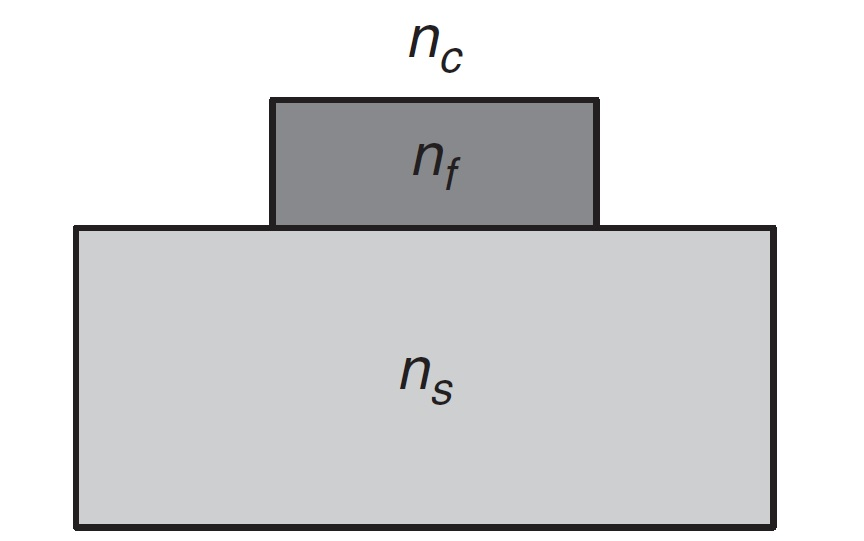
\includegraphics[width=\textwidth]{2-strip-wg}
		\caption{Strip waveguide}
		\label{fig:2_strip_wg}
	\end{subfigure}
	\hfill
	\begin{subfigure}[t]{0.3\textwidth}
		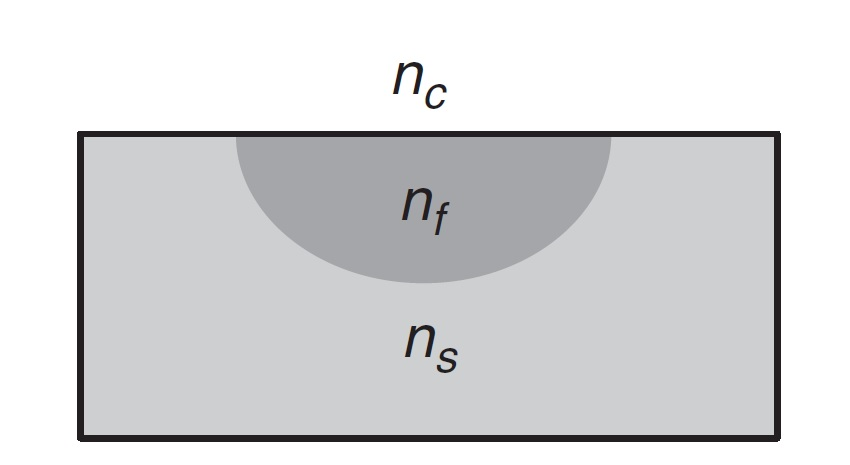
\includegraphics[width=\textwidth]{2-buried-wg}
		\caption{Buried waveguide}
		\label{fig:2_buried_wg}
	\end{subfigure}
	\caption{Different kinds of design for channel waveguides}
\end{figure}
\begin{itemize}	
	\item \textbf{Design rules of rib waveguides:} While designing these waveguides each of these have specific design rules for optimum performance and low-loss coupling, which has been standardized after years of research \cite{reed_silicon_2008}. The \gls{smc} for \textit{rib waveguides} is as follows:	
	\begin{equation}\label{eq:smc_rib_wg}
	\begin{aligned}
	\dfrac {W} {H}\leq 0.3+\dfrac {r} {\sqrt {1-r^{2}}},  && \text{ for } (0.5 \leq r < 1)
	\end{aligned}
	\end{equation}
	where $W$=waveguide width, $H$=rib height, $r$ is ratio of slab height to overall rib height.
	\begin{figure}[H] %h
		\centering
		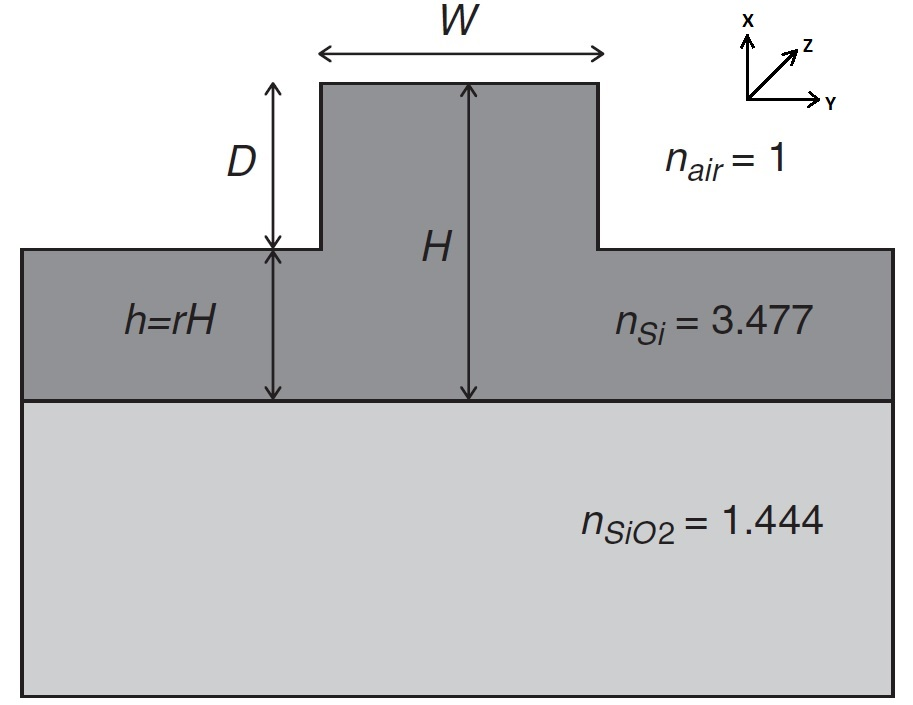
\includegraphics[width=0.75\textwidth]{2-rib-wg-design}
		\caption{Rib waveguide design rules}
		\label{fig:2_rib_wg_design}
	\end{figure}
	The main requirements of the waveguide to cater the propagation of waves is that the dimension of the waveguide has to be more than the wavelength of the propagating wave. However, depending on the required structure the design rules may change which can be found using simulation. 
	
	\item \textbf{Design rules of strip waveguides:} In mode confinement of light in optical waveguides the effective mode \gls{ri} is important. Strip waveguides offer more high \gls{ri} contrast in comparison to Rib waveguides. This can help in realization of ultra-dense photonic circuits because of high effective mode confinement. This can also achieve small bends which can improve the characterization of different monolithic optical circuits. In general a mix of rib and strip waveguides are used to achieve the desired circuitry, since sometimes the side walls cannot be etched in a perfectly smooth way causing greater evanescent fields from the waveguides introducing unnecessary coupling and losses. Using simulation for the desired scenario the robust values of the dimensions can be achieved.
\end{itemize}
	
		\subsection{Confinement factor}
Often it is necessary to know the confined power inside the core of the waveguide which helps in figuring out the waveguide mode. The confinement is also a measure of the proportion of the power in a given mode that lies within the core \cite{reed_silicon_2008}.  
\begin{equation}\label{eq:per}
\text{ Confinement factor } = \dfrac {\int _{-H / 2}^{H/2}E_{x}^{2}\left( y\right) dy} {\int _{-\infty }^{\infty }E_{x}^{2}\left( y\right) dy}
\end{equation}
Confinement factor is an important measure which is function of various factors like polarization, \gls{ri} difference between the core and cladding, mode number etc.	
		
		\subsection{Jones calculus}
Polarized light can be represented using Jones calculus. Polarized light is represented using \textit{Jones vector} and linear optical elements are represented by \textit{Jones matrices}.	When light crosses an optical element the resulting polarization of the emerging light is found by taking the product of the Jones matrix of the optical element and the Jones vector of the incident light. \textit{Jones calculus} is only applicable to light that is \textbf{already fully polarized} \cite{burch_introduction_1975}.
		
			\subsubsection{Jones vector}
The Jones vector describes the polarization of light in free space or another homogeneous isotropic non-attenuating medium, where the light can be properly described as transverse waves \cite{burch_introduction_1975}. The Jones vector is a complex vector that is a mathematical representation of a real wave. A typical representation of the electric field for the optical wave described in \ref{eq:wave_sol_electric} can be as follows:
\begin{equation}\label{eq:jones_vector}
E = \left( \begin{matrix} E_{x}\left( t\right) \\ E_{y}\left( t\right) \\ 0\end{matrix} \right) = \left( \begin{matrix} E_{x}e^{i\left( kz-\omega t+\phi _{x}\right)} \\ E_{y}e^{i\left( kz-wt+\phi _{y}\right) }\\ 0\end{matrix} \right) = \left( \begin{matrix} E_{x}e^{i\phi_x}\\ E_{y}e^{i\phi_y}\\ 0 \end{matrix} \right)e^{i\left( kz-\omega t\right)} 
\end{equation}
where $\phi_x$ and $\phi_y$ indicate the phasor notation. The Jones vector of the plane wave is described by:
\begin{equation}\label{eq:jones_vector_form}
\left( \begin{matrix} E_{x}e^{i\phi_x}\\ E_{y}e^{i\phi_y}\end{matrix} \right) 
\end{equation}
and the intensity of the optical, $I$ wave can be written as,
\begin{equation}\label{eq:jones_vector_intensity}
I = \left| E_x\right| ^{2}+\left| E_y\right| ^{2} 
\end{equation}
Generally, when considering Jones vector a wave of unit intensity is required for the consideration polarization, so Jones vector is noted using an unit vector where,
\begin{equation}\label{eq:jones_unit_vector_form}
	E\overline {E} = 1
\end{equation}
where $\overline {E}$ is the complex conjugate of $E$. 
In general the Jones representation of a normalized elliptically polarized beam with azimuth $\theta$ and elliptical angle $\epsilon$ is given by,
\begin{equation}\label{eq:jones_vector_general_form}
e^{i\phi}\left(\begin{matrix} 
\cos\theta\cos\epsilon - j\sin\theta\sin\epsilon\\
\sin\theta\cos\epsilon - j\cos\theta\sin\epsilon 
\end{matrix} \right) 
\end{equation}
where $e^{i\phi}$ is an arbitrary phase vector and $\phi = \phi_x - \phi_y$. So, for example a linear polarization of \gls{te} mode can be represented as,
\begin{equation}\label{eq:jones_vector_linear_pol}
\left(\begin{matrix}  
1 \\
0
\end{matrix} \right) 
\end{equation}
since, $\theta=0$ and $\epsilon = 0$.
			
			\subsubsection{Jones matrix}
Jones matrix are the formal representation of the various optical elements such as lenses, beam splitters, mirrors, phase retarders, polarizers at arbitrary angles that can modify polarization. They generally operate on Jones vector and helps in comprehend situations which light encounters multiple polarization elements in sequence. In these situations the products of the Jones matrices can be used to represent the transfer matrix. This situation can be represented using,
\begin{equation}\label{eq:jones_matrix}
[E_{output}] = J_{system}[E_{input}] 
\end{equation}
where $E_input$ is the input field into the optical system and $E_output$ is the generated output field represented using Jones vector. The matrix $J_system$ is the Jones matrix of the optical system comprising of a series of polarization devices. If there are $N$ devices in the system then the final transfer matrix comes out as,
\begin{equation}\label{eq:jones_transfer_matrix}
J_{system} =J_{N}J_{N-1}\ldots \ldots J_{2}J_{1} 
\end{equation}   
where $J_{N}$ is the Jones matrix for $n^{th}$ polarizing optical element.

		\subsection{Jones matrix for polarizing optical systems}
			\subsubsection{Polarizer}
			\subsubsection{Wave plate}
			
		\subsection{Poincaré sphere and state of polarization}
To view a complete representation of all the polarization ellipses generated using Jones vectors, a spherical structure with unit radius is used, which is known as Poincaré sphere. If the orientation in space of of the ellipse of polarization is determined by the azimuth, $\theta$ and ellipticity, $\epsilon$ then that point can be completely characterized by its longitude $2\theta$ and latitude $2\epsilon$. The north and south poles represent the right-handed and left-handed circular polarization respectively. In general the diametrically opposite points represent pairs of orthogonal polarization. The \gls{sop} and its corresponding location in the Poincaré sphere is visualized in the Fig. \ref{fig:2_poincare}. To go from one \gls{sop} to another the polarized light can be passed through various optical components which can be computed using the Jones matrix and the corresponding \gls{sop} can be depicted on the Poincaré sphere as well.     
\begin{figure}[H]
	\centering
	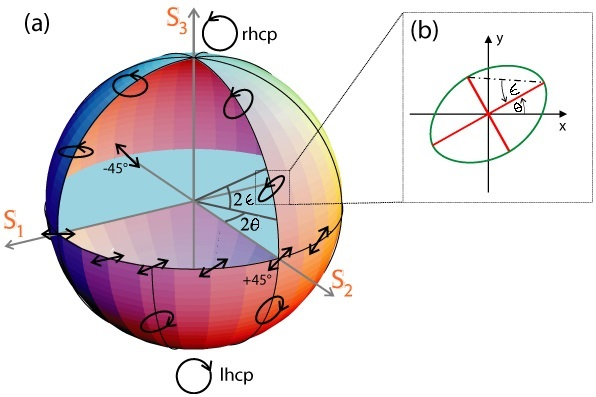
\includegraphics[width=0.75\textwidth]{2-poincare}
	\caption{(a) Representation of the Poincaré sphere (b) Representation of the ellipse parameters \cite{flossmann_stokes_2006}}
	\label{fig:2_poincare}
\end{figure}
\noindent The \gls{sop} of any wave is also defined using \gls{per} and polarization phase, $\phi$ given by the following equations:
\begin{equation}\label{eq:wave_sop}
\begin{aligned}
PER_{TE-TM} = 10\log \dfrac {P_{TM}} {P_{TE}}\\
PER_{TM-TE} = 10\log \dfrac {P_{TE}} {P_{TM}}\\
\phi =\phi _{x}-\phi _{y}
\end{aligned}
\end{equation}
For complete polarized light, the point on the Poincaré sphere must be fixed on time which requires,
\begin{equation}\label{eq:polarization_condition_1}
\dfrac {E_{x}\left( t\right) } {E_{y}\left( t\right) }=constant
\end{equation}
and,
\begin{equation}\label{eq:polarization_condition_2}
\phi = \phi_{x}(t) - \phi_{y}(t)=constant
\end{equation}
		\subsection{Stoke's parameter} 		
Quasi-monochromatic waves are mathematically treated using Stokes parameters ($S_0,S_1,S_2,S_3$), which constitute a vector generally known as Stokes vectors. Stokes vectors are used to keep track of the partial polarization (and attenuation) of a light beam in terms of total intensity (I), degree of polarization (p) and ellipse parameters, as the light progresses through an optical system. A Stokes vector can generally be represented as,
\begin{equation}\label{eq:stokes_vector}
\overrightarrow {S} = \left(\begin{matrix}  
	S_0 \\
	S_1 \\
	S_2 \\
	S_3
\end{matrix} \right) 
\end{equation}
where,
\begin{equation}\label{eq:stokes_parameters}
\begin{aligned}
\begin{cases}
S_{0}=I\\ 
S_{1}=I_{p}\cos 2\theta \cos 2\epsilon \\
S_{2}=I_{p}\sin 2\theta \cos 2\epsilon \\
S_{3}=I_{p}\sin 2\epsilon
\end{cases}
\end{aligned}
\end{equation}
Here, $I_p, 2\theta, 2\epsilon$ are the spherical coordinates of the 3-D vector of Cartesian coordinates $(S_1,S_2,S_3)$. So, given the Stokes parameters, the spherical coordinates $(p,2\theta,2\epsilon)$ can be obtained and represented by a point inside the Poincaré sphere using the following:
\begin{equation}\label{eq:stokes_spherical_coordinates}
\begin{aligned}
\begin{cases}
I = S_{0}\\ 
p = \dfrac {\sqrt {S_{1}^{2}+S_{2}^{2}+S_{3}^{2}}} {S_{0}} \\
2\theta = \tan^{-1}\dfrac {S_{2}} {S_{1}} \\
2\epsilon = \tan ^{-1}\dfrac {S_{3}} {\sqrt {S_{1}^{2}+S_{2}^{2}}}
\end{cases}
\end{aligned}
\end{equation}
The prescribed notations are portrayed on the Poincaré sphere in the following Fig. \ref{fig:2_stoke_param_poincare_sphere}.    
\begin{figure}[H]
	\centering
	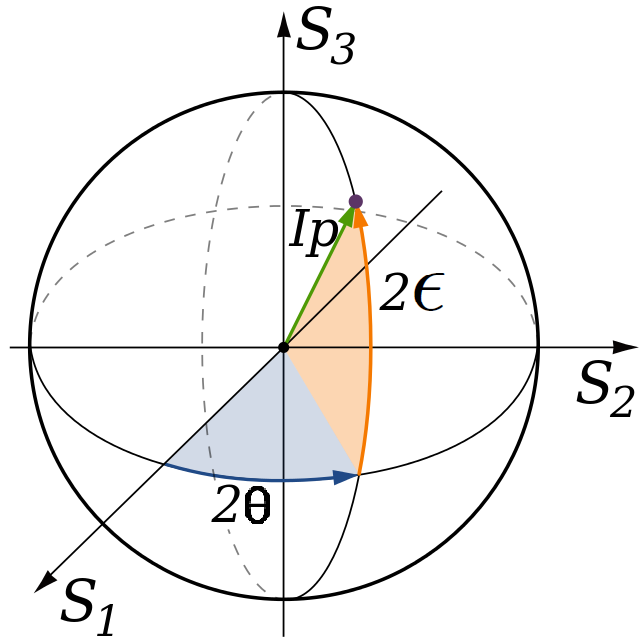
\includegraphics[width=0.75\textwidth]{2-stoke-param-poincare-sphere}
	\caption{Poincaré sphere, on or beneath which the three Stokes parameters [S1, S2, S3] are plotted in Cartesian coordinates \cite{stoke_poincare_parameter}}
	\label{fig:2_stoke_param_poincare_sphere}
\end{figure}
		
	\section{Theoretical background of MEMS}
	
		\subsection{Overview}
		
		\subsection{Actuation principle}
			
	\section{Polarization rotator}
	
		\subsection{Passive polarization rotator}
	
		\subsection{Active polarization rotator}
\end{document}
